\begin{figure}[h] 
\centering 
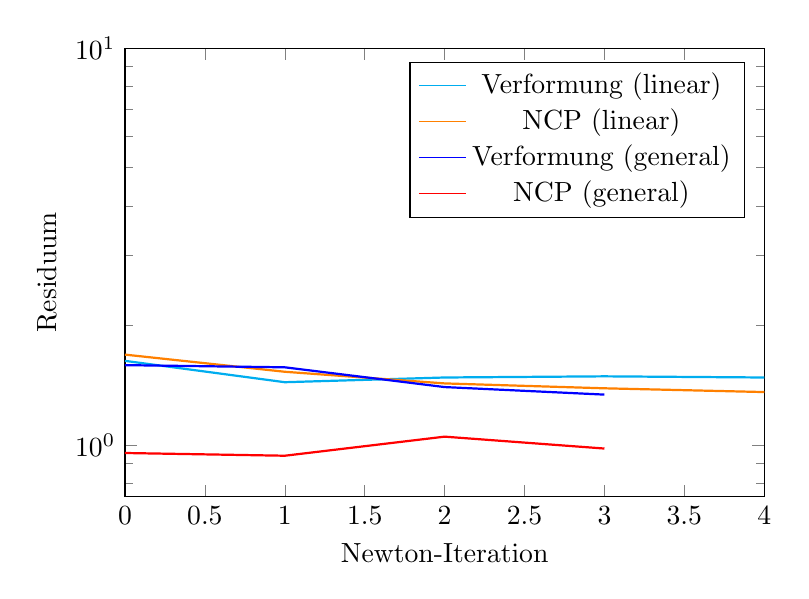
\begin{tikzpicture}[every plot/.append style={thick}] 
\begin{axis}[ 
label style={font=\normalsize}, 
xlabel={Newton-Iteration}, 
ylabel={Residuum}, 
xmin=0, xmax=4, 
ymode=log, 
ymin=0, ymax=10, 
width=0.8\textwidth, 
height=0.6\textwidth, 
legend pos=north east, 
legend style={cells={align=left}}, 
grid style=dashed, 
] 
\addplot[ 
color=cyan, 
] 
coordinates { 
(0, 1.63e+00)(1, 1.44e+00)(2, 1.48e+00)(3, 1.49e+00)(4, 1.48e+00)(5, 1.46e+00)(6, 1.43e+00)(7, 1.29e+00)(8, 1.25e+00)(9, 9.61e-01)(10, 7.82e-01)(11, 6.61e-01)(12, 6.60e-01)(13, 5.80e-01)(14, 5.73e-01)(15, 6.42e-01)(16, 6.40e-01)(17, 3.74e-01)(18, 3.59e-01)(19, 3.54e-01)(20, 3.60e-01)(21, 3.51e-01)(22, 5.39e-01)(23, 5.21e-01)(24, 4.55e-01)(25, 4.26e-01)(26, 4.83e-01)(27, 4.84e-01)(28, 3.65e-01)(29, 3.18e-01)(30, 3.16e-01)(31, 3.09e-01)(32, 2.94e-01)(33, 2.93e-01)(34, 2.93e-01)(35, 4.02e-01)(36, 3.93e-01)(37, 3.86e-01)}; 
\addlegendentry{Verformung (linear)} 
\addplot[ 
color=orange, 
] 
coordinates { 
(0, 1.69e+00)(1, 1.53e+00)(2, 1.43e+00)(3, 1.39e+00)(4, 1.36e+00)(5, 1.34e+00)(6, 1.30e+00)(7, 1.14e+00)(8, 1.19e+00)(9, 9.42e-01)(10, 4.71e-01)(11, 3.53e-01)(12, 3.48e-01)(13, 2.61e-01)(14, 2.28e-01)(15, 2.25e-01)(16, 1.69e-01)(17, 5.66e-19)(18, 5.64e-19)(19, 3.99e-19)(20, 7.00e-19)(21, 5.94e-19)(22, 1.25e-04)(23, 2.23e-04)(24, 1.67e-04)(25, 2.82e-05)(26, 2.78e-05)(27, 2.43e-05)(28, 7.50e-19)(29, 5.43e-19)(30, 5.76e-19)(31, 4.49e-19)(32, 4.94e-19)(33, 4.76e-19)(34, 3.05e-19)(35, 5.45e-19)(36, 4.48e-19)(37, 5.02e-19)}; 
\addlegendentry{NCP (linear)} 
\addplot[ 
color=blue, 
] 
coordinates { 
(0, 1.59e+00)(1, 1.57e+00)(2, 1.40e+00)(3, 1.34e+00)}; 
\addlegendentry{Verformung (general)} 
\addplot[ 
color=red, 
] 
coordinates { 
(0, 9.55e-01)(1, 9.40e-01)(2, 1.05e+00)(3, 9.80e-01)}; 
\addlegendentry{NCP (general)} 
\end{axis} 
\end{tikzpicture} 
\caption{Residuen des Stoffgesetzes 'St.Venant' mit Hinderniss 'Hut' und 2178 Freiheitsgraden für die Verschiebung.} 
\label{fiq:St.Venant_Hut_level4} 
\end{figure} 
